\addtocontents{toc}{\protect\setcounter{tocdepth}{0}}
\hypersetup{bookmarksdepth=0}
\chapter{Funcionament de l'eye-tracker}\label{sec:tobii}

Utilitzem l'eye-tracker Tobii Pro Spectrum, que registra la zona de la pantalla que mira el participant a 600~Hz.
El programari Tobii Pro Lab calcula les fixacions i permet definir cada paraula d'un text com una àrea d'interès (AOI, per les sigles en anglès).
El programari permet calcular algunes mètriques, però presenta limitacions en aspectes com el càlcul de regressions.
Per això exportem les dades i calculem les mètriques d'eye-tracking---FFD, TFD, FC i regressions---de manera independent.

El problema és que Tobii Pro Lab no optimitza el format d'exportació.
En comptes de crear un fitxer per a cada text, crea un fitxer amb tots els instants com a files i totes les AOI com a columnes.
Per tant, la mida del fitxer creix quadràticament amb el nombre de texts i el programa es bloqueja.
Per optimitzar aquest procés, vam exportar diversos fitxers de la manera següent\footnote{Dins del menú Analyze/Data export}. Sempre vam utilitzar el filtre \textit{Tobii I-VT (Fixation)} i l'opció \textit{noise reduction}, tant per a l'obertura de l'ull com per al diàmetre de la pupil·la:

\begin{enumerate}
    \item \textbf{Dades generals}: inclouen el dia, l'hora i els resultats del calibratge. Es van seleccionar el grup General, excepte AOI size, timestamp i event value; un sol Time of interest i cap AOI.
    \item \textbf{Anotacions}: inclouen les entrades de teclat dels participants. Es van seleccionar Participant name, Event i Event value; Times of Interest = Media gaze data i cap AOI.
    \item \textbf{Dades del sensor}: cal seleccionar grups petits d'AOI i els temps corresponents a Times of interest. Finalment, es van crear quatre grups de 10 texts per participant. Es poden exportar simultàniament en fitxers individuals amb \textit{Format=multiple standard files}. Després, vam convertir els fitxers exportats al format \textit{parquet}, més eficient.
        \begin{itemize}
            \item General: Participant name
            \item Eye tracking data: Pupil diameter, Validity of eye data
            \item Media: stimulus name
            \item Eye movement events: eye movement type, duration and index, fixation point, AOI hit
        \end{itemize}
\end{enumerate}


\chapter{TFD i regressions}\label{app:tfd}

\section{Durada total de fixació (TFD)}

La durada total de fixació (\textit{Total Fixation Duration}, TFD) mesura l'atenció acumulada en una AOI al llarg de tota la lectura.
Es calcula com la suma de les durades de totes les fixacions que cauen dins d'una AOI concreta.
En el nostre cas, la normalitzem pel temps total de fixació de cada text:

\[
\text{TFD}_{i} = \frac{\sum_{k \in \text{fixacions}_i} d_k}{\sum_{j=1}^{N} \sum_{k \in \text{fixacions}_j} d_k}
\]

on $d_k$ és la durada de la fixació $k$, $i$ és l'índex del token (AOI) i $N$ és el nombre total de tokens del text.
Aquesta normalització ens permet comparar patrons d'atenció entre participants amb velocitats de lectura diferents.
Una TFD més alta en un token indica que els participants hi dediquen proporcionalment més temps d'atenció total.
En contexts de sexisme, una TFD més alta en paraules amb càrrega emotiva o ideològica pot indicar un processament més profund del contingut discriminatori.

\section{Regressions}

Una regressió ocorre quan la mirada es desplaça cap enrere---de dreta a esquerra en texts escrits d'esquerra a dreta---respecte de la posició actual de lectura.
Les regressions són un fenomen cognitiu ben documentat en la recerca sobre lectura~\cite{rayner1998eye, rayner2009eye} i reflecteixen processos de reprocessament, verificació o resolució d'ambigüitat.
Se'n distingeixen dos tipus.
Les regressions intralínia (\textit{within-line}) es produeixen quan el lector mou la mirada dins de la mateixa línia cap a un token anterior. S'associen principalment a dificultats de comprensió local, com ara paraules amb diversos significats o estructures sintàctiques complexes.
Les regressions interlínia (\textit{between-line}) es produeixen quan la mirada salta a una línia anterior. Es relacionen amb processos de coherència global, com ara connectar informació prèvia amb el contingut actual.

La taxa de regressió es defineix com la proporció de sacades que són regressions respecte al total de sacades:

\[
r = \frac{n_{\text{regressions}}}{n_{\text{sacades}}} = \frac{n_{\text{regressions}}}{n_{\text{fixacions}} - 1}
\]

En condicions normals de lectura, la taxa de regressió se situa entre el 10\% i el 15\% del total de sacades~\cite{rayner2009eye}.
Taxes més altes indiquen fragments que generen més dificultat de processament.
Aquestes mètriques s'han utilitzat àmpliament en estudis sobre processament de frases i ambigüitat sintàctica. Per exemple, \textcite{alvarez2025} mostren que les regressions són especialment informatives per identificar les regions que generen dificultat en parlants de català L1 i anglès L2.

En l'anàlisi de regressions, fem servir les definicions de \textit{regression-to} i \textit{regression-from}~\cite{rayner2009eye}.
El token de destí és aquell cap al qual es dirigeix la regressió i indica on torna el lector per reprocessar la informació. El token d'origen és aquell des del qual es produeix la regressió i indica on interromp el lector la lectura per tornar enrere.
Per exemple, si un participant està llegint el token $t_{10}$ i fa una regressió cap al token $t_{5}$, aquesta es registra com $\text{FROM} = t_{10}$, $\text{TO} = t_{5}$.
Aquesta convenció (\textit{regression-to} / \textit{regression-from}) és estàndard en la literatura sobre eye-tracking i lectura~\cite{rayner2009eye}.
En el context del sexisme, les regressions poden indicar moments en què el lector torna a processar contingut discriminatori o irònic. Això pot ajudar a identificar regions que generen confusió o conflicte cognitiu.

Per identificar els tokens significatius, fem servir un test de permutació.
Per a cada parell (participant, text), permutem aleatòriament l'ordre de la seqüència de fixacions, però mantenim la distribució global de fixacions per token. Així generem una distribució nul·la en què les regressions són aleatòries i la comparem amb les observades per determinar quins tokens reben més regressions de les esperables per atzar.

% \chapter{Visualització spans}\label{sec:spans_viz}
%
% Per visualitzar diversos segments, utilitzem un script basat en la biblioteca spaCy\footnote{https://spacy.io/}.

\chapter{Calibratge i validació}\label{app:calibration}

Per a tots els participants, es va fer una calibració inicial amb 9 punts d'entrenament i 4 de validació.
La \autoref{tab:calibration} presenta les mètriques de calibratge i validació de l'eye-tracker Tobii Pro Spectrum per a cada participant.

\iftables
\begin{table}[htbp]
\small
\centering
\begin{tabular}{llcc}
\toprule
\textbf{Participant} & \textbf{Sexe} & \textbf{Precisió Calibratge (mm)} & \textbf{Precisió Validació (mm)} \\
\midrule
M1 & home & 1,7 & 2,9 \\
M2 & home & 2,3 & 7,5 \\
M3 & home & 1,0 & 2,8 \\
M4 & home & 1,7 & 2,8 \\
M5 & home & 1,2 & 4,4 \\
F1 & dona & 1,2 & 12,5 \\
F2 & dona & 1,2 & 5,6 \\
F3 & dona & 1,3 & 5,1 \\
F4 & dona & 3,8 & 6,2 \\
F5 & dona & 1,5 & 5,7 \\
\bottomrule
\end{tabular}
\caption{Precisió de calibratge i validació de l'eye-tracker per participant (en mil·límetres). Els valors més baixos indiquen una qualitat de calibratge millor.}
\label{tab:calibration}
\end{table}
\fi

La majoria dels participants presenten una precisió de calibratge adequada ($\leq$ 2,3~mm).
Les participants F1 i F4 mostren una precisió de validació pitjor (12,5 i 6,2~mm, respectivament).
Tot i això, els seus patrons de lectura permeten identificar quina paraula miren en cada moment.

En canvi, tot i presentar una precisió de validació de 5,6~mm, les dades de F2 no són tan clares. En alguns casos sembla que llegeixi entre línies o fins i tot la línia equivocada.
Per això vam avaluar l'impacte d'excloure-la de l'anàlisi.
La \autoref{tab:exclusion_comparison} compara les mètriques principals amb les seves dades i sense.

\iftables
\begin{table}[htbp]
\small
\centering
\begin{tabular}{lrrr}
\toprule
\textbf{Mètrica} & \textbf{Amb F2 (10)} & \textbf{Sense F2 (9)} & \textbf{Delta} \\
\midrule
Spearman (vs.\ segments) & $+0,036$ & $+0,047$ & $+0,010$ \\
JS (vs.\ segments) & 0,257 & 0,256 & $-0,000$ \\
\bottomrule
\end{tabular}
\caption{Comparació de mètriques de distribució F2 i sense. Els valors són promitjats sobre els 40 texts.}
\label{tab:exclusion_comparison}
\end{table}
\fi

Les diferències són negligibles: la correlació de Spearman canvia en 0,01 i la divergència JS en menys de 0,001.
La prova per a mostres aparellades, aplicada per text, no mostra diferències significatives ni per a Spearman ($p = 0,47$) ni per a la JS ($p = 0,11$).
Concloem que l'exclusió de la participant F2 no altera substancialment els resultats de l'anàlisi.
Per tant, conservem les seves dades en tots els resultats.

\chapter{Prominència per categories gramaticals}\label{sec:pos_analysis}

Seguint l'anàlisi de \textcite{ikhwantriLookingDeepEyes2023}, comparem la distribució de prominència dels models segons les categories gramaticals amb l'atenció humana (TFD).
Per a cada text, calculem la TFD mitjana dels 10 participants, etiquetem els tokens amb spaCy\footnote{https://spacy.io/} (\texttt{es\_core\_news\_sm}), sumem la prominència---o la TFD---dels tokens de cada categoria i normalitzem els valors perquè sumin 1,0.
La \autoref{fig:pos_distribution} mostra la distribució del model més ben alineat (BETO LRP), del menys ben alineat (MrBERT-es IG) i de l'atenció humana (TFD).

\begin{figure}[htbp]
\centering
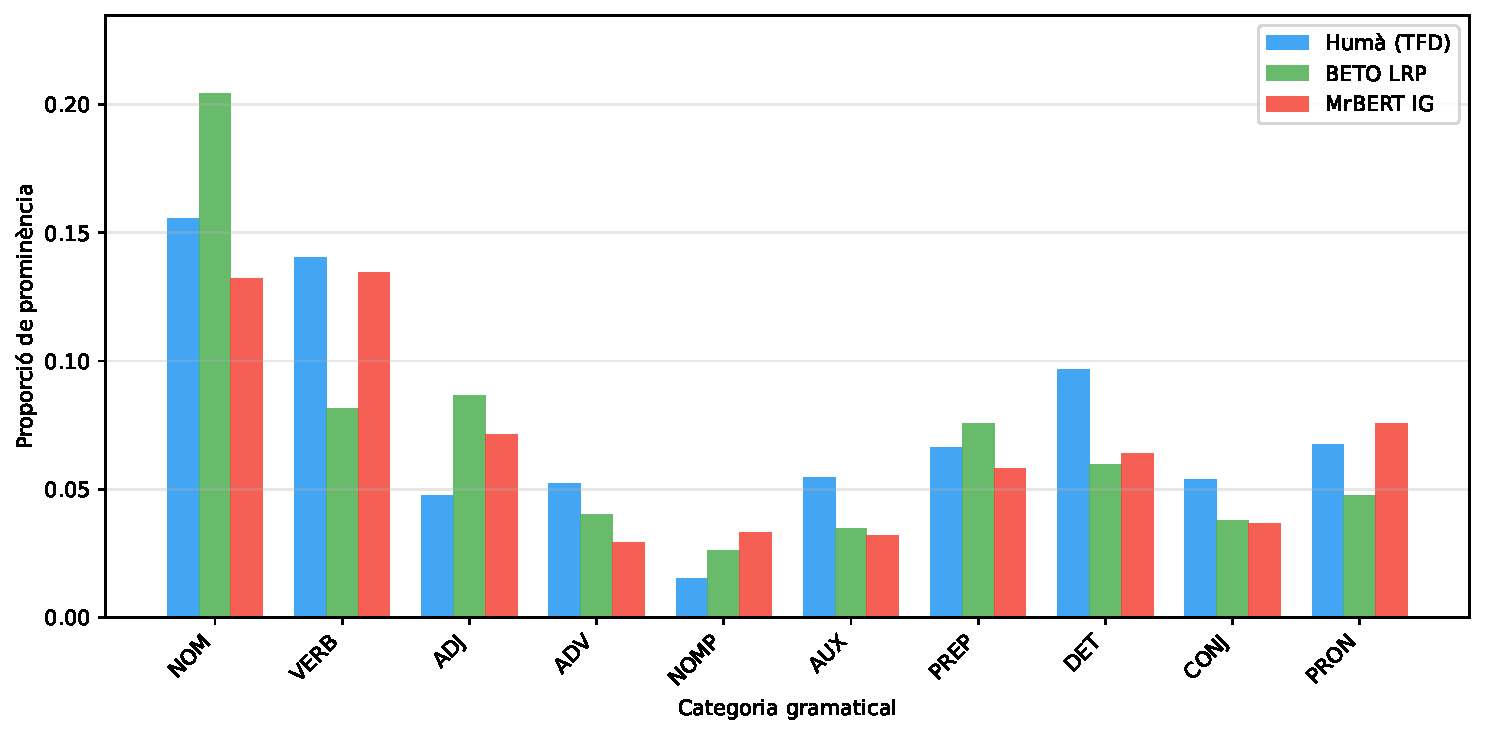
\includegraphics[width=0.85\textwidth]{figures/pos_saliency_distribution.pdf}
\caption{Distribució de prominència per categoria gramatical: atenció humana (TFD) vs.\ millor model (BETO LRP) i pitjor model (MrBERT-es IG).}
\label{fig:pos_distribution}
\end{figure}

Els resultats mostren divergències entre els models i l'atenció humana.
Els lectors dediquen una proporció més alta de la seva atenció als determinants (\textit{DET}: 9,7\% vs.\ 6,0\%--6,4\%) i als auxiliars (\textit{AUX}: 5,5\% vs.\ 3,2\%--3,5\%), dues categories funcionals que els models subvaloren.
En canvi, BETO LRP sobrevalora els noms (\textit{NOM}: 20,4\% vs.\ 15,5\%) i els adjectius (\textit{ADJ}: 8,6\% vs.\ 4,7\%). Això suggereix que el model centra la prominència en elements lèxics de contingut, mentre que els lectors la distribueixen més entre les categories gramaticals.
MrBERT-es IG presenta una distribució més propera a la humana en els noms (13,2\%), però subvalora els verbs (\textit{VERB}: 13,4\% vs.\ 14,0\%).
Tots dos models subvaloren els adverbis (\textit{ADV}: 2,9\%--4,0\% vs.\ 5,2\%).
Aquests resultats són coherents amb els d'Ikhwantri et al., que observen que els models tendeixen a sobreponderar els adjectius i els noms en comparació amb els humans.

\chapter{Ablació del filtratge de paraules buides}\label{sec:stopword_ablation}

Avaluem l'impacte del filtratge de paraules buides (\textit{stopwords}) sobre les mètriques de distribució, utilitzant la TFD com a característica d'eye-tracking.
La \autoref{tab:stopword_ablation} mostra la divergència JS per a les tres parelles de distribucions (TFD--segments, models--segments i models--TFD), amb filtratge de paraules buides i sense.
El filtratge redueix la JS en tots els casos. L'efecte és més accentuat en la comparació TFD--segments (26,5\%), perquè les paraules buides reben una atenció similar dels lectors, però no contribueixen a discriminar entre zones sexistes i no sexistes.
L'efecte és menor, però consistent en les comparacions que inclouen els models (5,3\%--8,3\%), fet que confirma que el filtratge millora la discriminació en totes les parelles.
Per aquest motiu, totes les comparacions amb els models que presentem al capítol de resultats utilitzen distribucions amb les paraules buides filtrades.
\iftables
\begin{table}[htbp]
\small
\centering
\begin{tabular}{lccr}
\toprule
\textbf{Parella} & \textbf{JS (tots)} & \textbf{JS (filtrat)} & \textbf{$\Delta$} \\
\midrule
TFD–Segments (TFD)               & 0,137 & 0,100 & $-26,5$\% \\
Model–Segments (BETO LRP)      & 0,827 & 0,768 & $-7,1$\% \\
Model–TFD (BETO LRP)           & 0,827 & 0,783 & $-5,3$\% \\
Model–Segments (MrBERT-es IG)     & 0,859 & 0,788 & $-8,3$\% \\
Model–TFD (MrBERT-es IG)          & 0,865 & 0,804 & $-7,0$\% \\
\bottomrule
\end{tabular}
\caption{Ablació: efecte del filtratge de paraules buides sobre la divergència JS per a les tres parelles de distribucions (TFD com a característica d'eye-tracking).}
\label{tab:stopword_ablation}
\end{table}
\fi
